\documentclass[a4paper]{article}
\usepackage[utf8]{inputenc}
\usepackage[T1]{fontenc}
\usepackage{graphics}
\usepackage{libertine}
\usepackage{tango}

\hypersetup{urlcolor=DarkChocolate}

\title{L'art du test}
%\author{\scalebox{0.35}{ \includegraphics{logo_azae}}}
\author{Thomas Clavier}
\date{}

\setlength{\parindent}{0pt}
\newcounter{question}
\setcounter{question}{1}
\newcommand{\q}{
  \textcolor{DarkOrange}{\textbf{Question \thequestion : }}
  \addtocounter{question}{1}
  \newline
}

\begin{document}

\maketitle

\section*{Test Driven Development}

Faire du développement piloté par les tests permet d'atteindre 3 objectifs :

\begin{itemize}
\item Contrôler et conserver la qualité du produit tout au long du projet
\item Se focaliser sur l'amélioration du code, plutôt que sur la correction des bugs
\item améliorer la productivité de l'équipe en automatisant un maximum de tâches redondantes et ennuyantes
\end{itemize}

Le déroulement des développements est le suivant :
\begin{itemize}
  \item écriture du test
  \item vérifier que le test est rouge
  \item commit
  \item implémenter la solution la plus simple pour faire passer le test au vert
  \item commit
  \item restructurer le code
  \item vérifier que tous les tests sont encore verts
  \item commit 
\end{itemize}

\begin{center}
\scalebox{0.7}{ 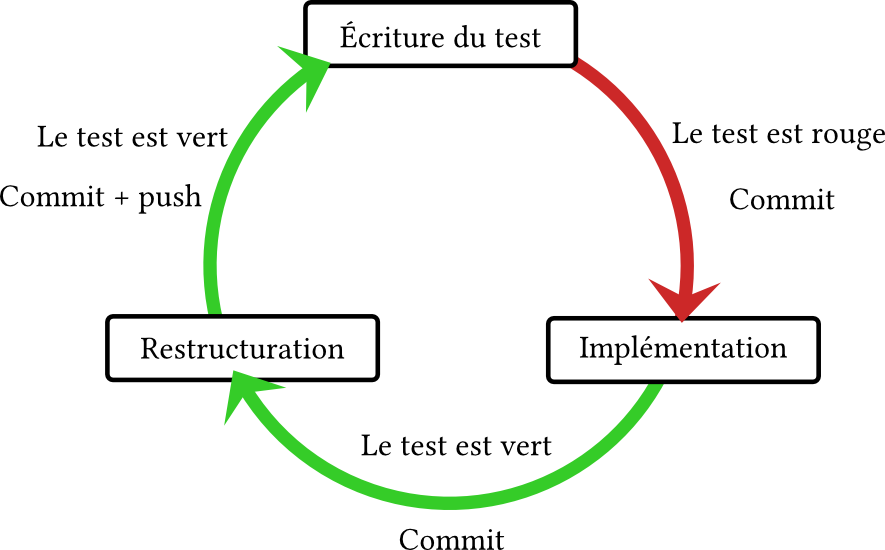
\includegraphics{tdd}}
\end{center}

\subsection*{À propos des tests}
Avec JUnit 4 il est possible d'utiliser des annotations : 
\begin{itemize}
  \item @Test pour définir une méthode "public void" comme une méthode de test.
  \item @Before pour lancer une méthode "public void" avant chaque test.
  \item @After pour lancer une méthode "public void" après chaque test.
\end{itemize}
Voir \url{https://github.com/junit-team/junit/wiki} pour toute la documentation.

Un test se décompose toujours en 3 parties : Given, When, Then. Dans le Then il est préférable de ne mettre qu'un seul assert.

Il est important de nommer le test avec un nom qui explique clairement l'intention fonctionnelle. Comme les phrases peuvent être longue l'utilisation d'une notation snake\_case est authorisé. C'est d'ailleurs le seul cas d'usage de cette notation dans la norme Oracle.

\begin{verbatim}
import org.junit.Test;
import org.junit.Assert;

...

@Test
public void num2text_should_return_zero_when_0_is_in_inut () {
  // Given
  Convert myConverter = new Convert();
  // When
  String text = Convert.num2text("0");
  // Then
  Assert.assertEquals("zero", text);
}
\end{verbatim}

\section*{Code propre}

Le code propre c’est du code :
\begin{itemize}
\item qui passe ses tests,
\item qui ne contient pas de redondance,
\item qui est explicite,
\item qui est minimal.
\end{itemize}

Nous passons plus de temps à lire du code qu’à en écrire. En rendant le
code facile à lire, nous le rendons plus facile à écrire.

Quelques règles de base : 
\begin{itemize}
  \item La règle du boy scout
  \item La ligne vide 
  \item pas de commentaire
  \item max 20 lignes par méthode
  \item moins de 3 niveaux d'indentation
  \item Utiliser des Exceptions et pas des valeurs spéciales
  \item Utiliser stdin, stdout et stderr
  \item Pas de variable globale
  \item Des noms de variables explicites
  \item Modulariser
  \item Couplage faible
\end{itemize}

\section*{Évaluation}
Le score sur le serveur n'est pas un critère d'évaluation, en revanche la propreté du code, la présence des tests et la rigueure de l'utilisation de git sont des critères d'évaluation.

\section*{Codons}
L’objectif du TP est de réaliser un convertisseur de chiffre romains

Créez un projet public et le référencer sur l'url au tableau et sur \url{https://github.com/tclavier/tp-tdd}.

Décompresser l’archive du projet dans votre workspace eclipse puis l’importer.
Dans le répertoire du projet ajouter le remote git vers votre projet public.
\begin{verbatim}
git remote add origin url
\end{verbatim}
avant de commiter et "pusher" votre travail.

\end{document}

